\begin{figure}[!htb]
\begin{center}
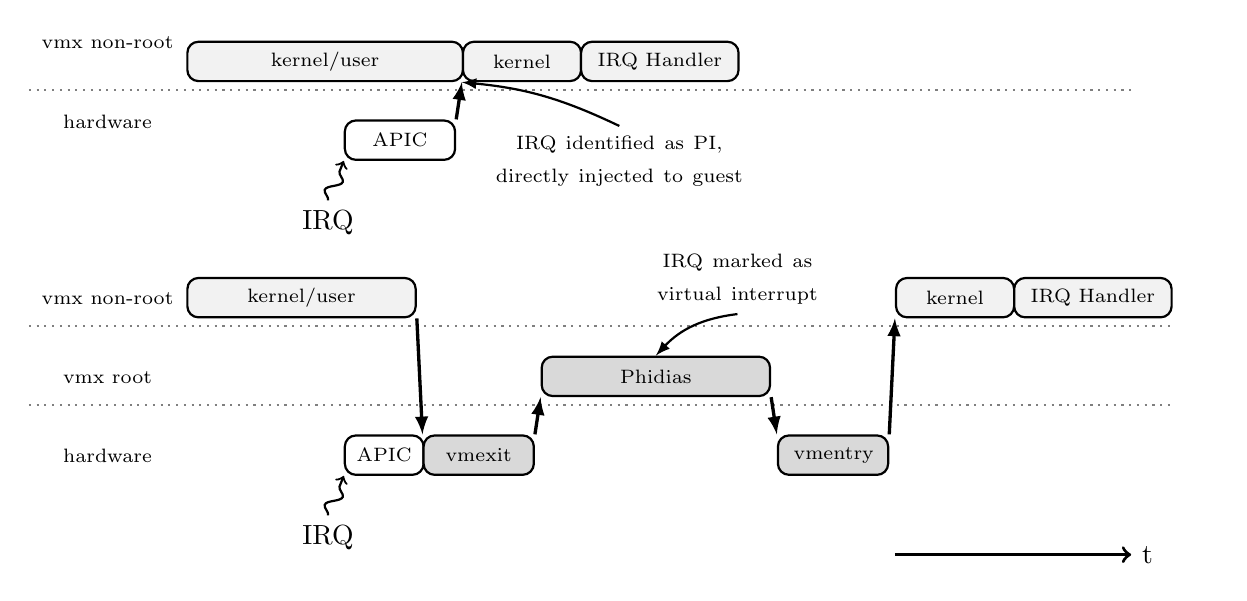
\begin{tikzpicture}

%\draw[step=1cm, gray, very thin, dotted] (-1,-1) grid (10,6);

\draw[black, very thick, ->] (9,-1) -- (12,-1) node [below, right] {t};
\draw[black, thick, dotted, opacity=0.5] (-2,0.9) -- (12.5,0.9) node at (13,0.9) [below] {};
\draw[black, thick, dotted, opacity=0.5] (-2,1.9) -- (12.5,1.9) node at (13,1.9) [below] {};
\node at (-1, 2.25) {\scriptsize{vmx non-root}};
\node at (-1, 1.25) {\scriptsize{vmx root}};
\node at (-1, 0.25) {\scriptsize{hardware}};


\node at (0,2) [rectangle, draw=black, thick, fill=black!5, rounded corners, minimum height = 0.5cm, minimum width = 2.9cm, anchor=south west] (kubefore) {\scriptsize{kernel/user}};
%\draw[black, thick, dashed, opacity=0.7] (1.95,-0.25) -- (1.95, 3.0)  node [above, text width = 1cm] {IRQ};
\node at (2,0) [rectangle, draw=black, thick, fill=white, rounded corners, minimum height = 0.5cm, minimum width = 1cm, anchor=south west] (apic) {\scriptsize{APIC}};
%\draw[black, thick, dashed] (3.0,-0.25) -- (3.0, 3.75)  node [above, text width = 4cm] {IRQ not marked as PI};
\node at (3,0) [rectangle, draw=black, thick, fill=black!15, rounded corners, minimum height = 0.5cm, minimum width = 1.4cm, anchor=south west] (vmexit) {\scriptsize{vmexit}};
\node at (4.5,1) [rectangle, draw=black, thick, fill=black!15, rounded corners, minimum height = 0.5cm, minimum width = 2.9cm, anchor=south west] (phidias) {\scriptsize{Phidias}};
\node at (7.5,0) [rectangle, draw=black, thick, fill=black!15, rounded corners, minimum height = 0.5cm, minimum width = 1.4cm, anchor=south west, text width=1cm] (vmentry) {\scriptsize{vmentry}};
%\draw[black, thick, dashed] (7.5,-0.25) -- (7.5, 3.25)  node [above, text width = 4cm] {IRQ marked pending};
\node at (9,2) [rectangle, draw=black, thick, fill=black!5, rounded corners, minimum height = 0.5cm, minimum width = 1.5cm, anchor=south west] (kafter) {\scriptsize{kernel}};
\node at (10.5,2) [rectangle, draw=black, thick, fill=black!5, rounded corners, minimum height = 0.5cm, minimum width = 2cm, anchor=south west] (irqhandler) {\scriptsize{IRQ Handler}};
\draw[thick, decorate, decoration=snake, ->] (1.8, -0.5) -- (2, 0) node at (1.8, -0.5) [below] {IRQ};


\node at (7,2.5) (irqvi) [text width=4cm, align=center] {\scriptsize{IRQ marked as virtual interrupt}};
\node at (5.5,4) (irqpi) [text width=4cm, align=center] {\scriptsize{IRQ identified as PI, directly injected to guest}};

\begin{scope}[>=latex]
	%\draw [thick, ->] (kubefore.south east) to [bend right=0] (vmexit.north west);
	\draw [very thick, ->] (kubefore.south east) -- (vmexit.north west);
	\draw [very thick, ->] (vmexit.north east) -- (phidias.south west);
	\draw [very thick, ->] (phidias.south east) -- (vmentry.north west);
	\draw [very thick, ->] (vmentry.north east) -- (kafter.south west);
	\draw [thick, ->] (irqvi.south) to [bend right=20] (phidias.north);
	
\end{scope}

\draw[black, thick, dotted, opacity=0.5] (-2,8-3.1) -- (12,8-3.1) node at (13,8-3.1) [below] {};
\node at (-1, 8-2.5) {\scriptsize{vmx non-root}};
\node at (-1, 8-3.5) {\scriptsize{hardware}};

\node at (0,8-3) [rectangle, draw=black, thick, fill=black!5, rounded corners, minimum height = 0.5cm, minimum width = 3.5cm, anchor=south west] (kubefore2) {\scriptsize{kernel/user}};
%\draw[black, thick, dashed, opacity=0.7] (1.95,-4.25) -- (1.95, -2.0)  node [above, text width = 1cm] {IRQ};
\draw[thick, decorate, decoration=snake, ->] (1.8, 8-4.5) -- (2, 8-4) node at (1.8, 8-4.5) [below] {IRQ};
\node at (2.0,8-4) [rectangle, draw=black, thick, fill=white, rounded corners, minimum height = 0.5cm, minimum width = 1.4cm, anchor=south west] (apic2) {\scriptsize{APIC}};
%\draw[black, thick, dashed] (3.5,-4.25) -- (3.5, -1.5)  node [above, text width = 4cm] {IRQ recognized as PI};

\node at (3.5,8-3) [rectangle, draw=black, thick, fill=black!5, rounded corners, minimum height = 0.5cm, minimum width = 1.5cm, anchor=south west] (kafter2) {\scriptsize{kernel}};
\node at (5.0,8-3) [rectangle, draw=black, thick, fill=black!5, rounded corners, minimum height = 0.5cm, minimum width = 2cm, anchor=south west] (irqhandler2) {\scriptsize{IRQ Handler}};

\begin{scope}[>=latex]
	\draw [very thick, ->] (apic2.north east) -- (kafter2.south west);
	\draw [thick, ->] (irqpi.north) to [bend right=10] (kafter2.south west);
\end{scope}


\end{tikzpicture}
\end{center}
\ifreport
\caption{Posted interrupt versus virtual interrupt delivery}
\fi
\label{fig-posted-interrupts}
\end{figure}
